\documentclass[review]{elsarticle}

\usepackage{lineno,hyperref}
\usepackage{graphicx}
\usepackage{amsmath}
\usepackage[linesnumbered,ruled]{algorithm2e}
\modulolinenumbers[5]

\journal{Expert Systems with Applications}

%%%%%%%%%%%%%%%%%%%%%%%
%% Elsevier bibliography styles
%%%%%%%%%%%%%%%%%%%%%%%
%% To change the style, put a % in front of the second line of the current style and
%% remove the % from the second line of the style you would like to use.
%%%%%%%%%%%%%%%%%%%%%%%

%% Numbered
%\bibliographystyle{model1-num-names}

%% Numbered without titles
%\bibliographystyle{model1a-num-names}

%% Harvard
%\bibliographystyle{model2-names.bst}\biboptions{authoryear}

%% Vancouver numbered
%\usepackage{numcompress}\bibliographystyle{model3-num-names}

%% Vancouver name/year
%\usepackage{numcompress}\bibliographystyle{model4-names}\biboptions{authoryear}

%% APA style
%\bibliographystyle{model5-names}\biboptions{authoryear}

%% AMA style
%\usepackage{numcompress}\bibliographystyle{model6-num-names}

%% `Elsevier LaTeX' style
\bibliographystyle{elsarticle-num}
%%%%%%%%%%%%%%%%%%%%%%%

\begin{document}

\begin{frontmatter}

\title{Origin based Order Independent Association Rule Mining using multiple OIMASP tree\tnoteref{mytitlenote}}
\tnotetext[mytitlenote]{Fully documented templates are available in the elsarticle package on \href{http://www.ctan.org/tex-archive/macros/latex/contrib/elsarticle}{CTAN}.}

%% Group authors per affiliation:
\author{Elsevier\fnref{myfootnote}}
\address{Radarweg 29, Amsterdam}
\fntext[myfootnote]{Since 1880.}

%% or include affiliations in footnotes:
\author[mymainaddress,mysecondaryaddress]{Elsevier Inc}
\ead[url]{www.elsevier.com}

\author[mysecondaryaddress]{Global Customer Service\corref{mycorrespondingauthor}}
\cortext[mycorrespondingauthor]{Corresponding author}
\ead{support@elsevier.com}

\address[mymainaddress]{1600 John F Kennedy Boulevard, Philadelphia}
\address[mysecondaryaddress]{360 Park Avenue South, New York}

\begin{abstract}
Association rule learning is a rule-based machine learning method for discovering interesting relations between variables in large databases.
\end{abstract}

\begin{keyword}
data-mining \sep Association Rule Mining \sep frequent-itemset mining 
\end{keyword}

\end{frontmatter}

\section{Introduction}
Association rule mining is a rule-based machine learning procedure to find interesting patterns in the transaction database based on individual and conditional frequencies. In the traditional approach, two steps are involved in generating rules. First, generate all frequent itemsets and pruned non-frequent ones and then in the second stage rules are derived from those frequent itemsets. An association rule e.g. \{bread, milk\} $\Rightarrow$ \{butter\} in market basket analysis means if one purchase bread and milk together it is highly likely that they will also buy butter. Apart from market basket analysis, association rule mining is useful in intrusion detection, bioinformatics, and many other applications.

In 2014 O. M. Soyal \cite{oldmasp} proposed a new approach to extract mostly associated sequential patterns (MASPs) using less computational resources in terms of time and memory while generating a long sequence of patterns that have the highest co-occurrence.

\begin{figure}
\begin{center}
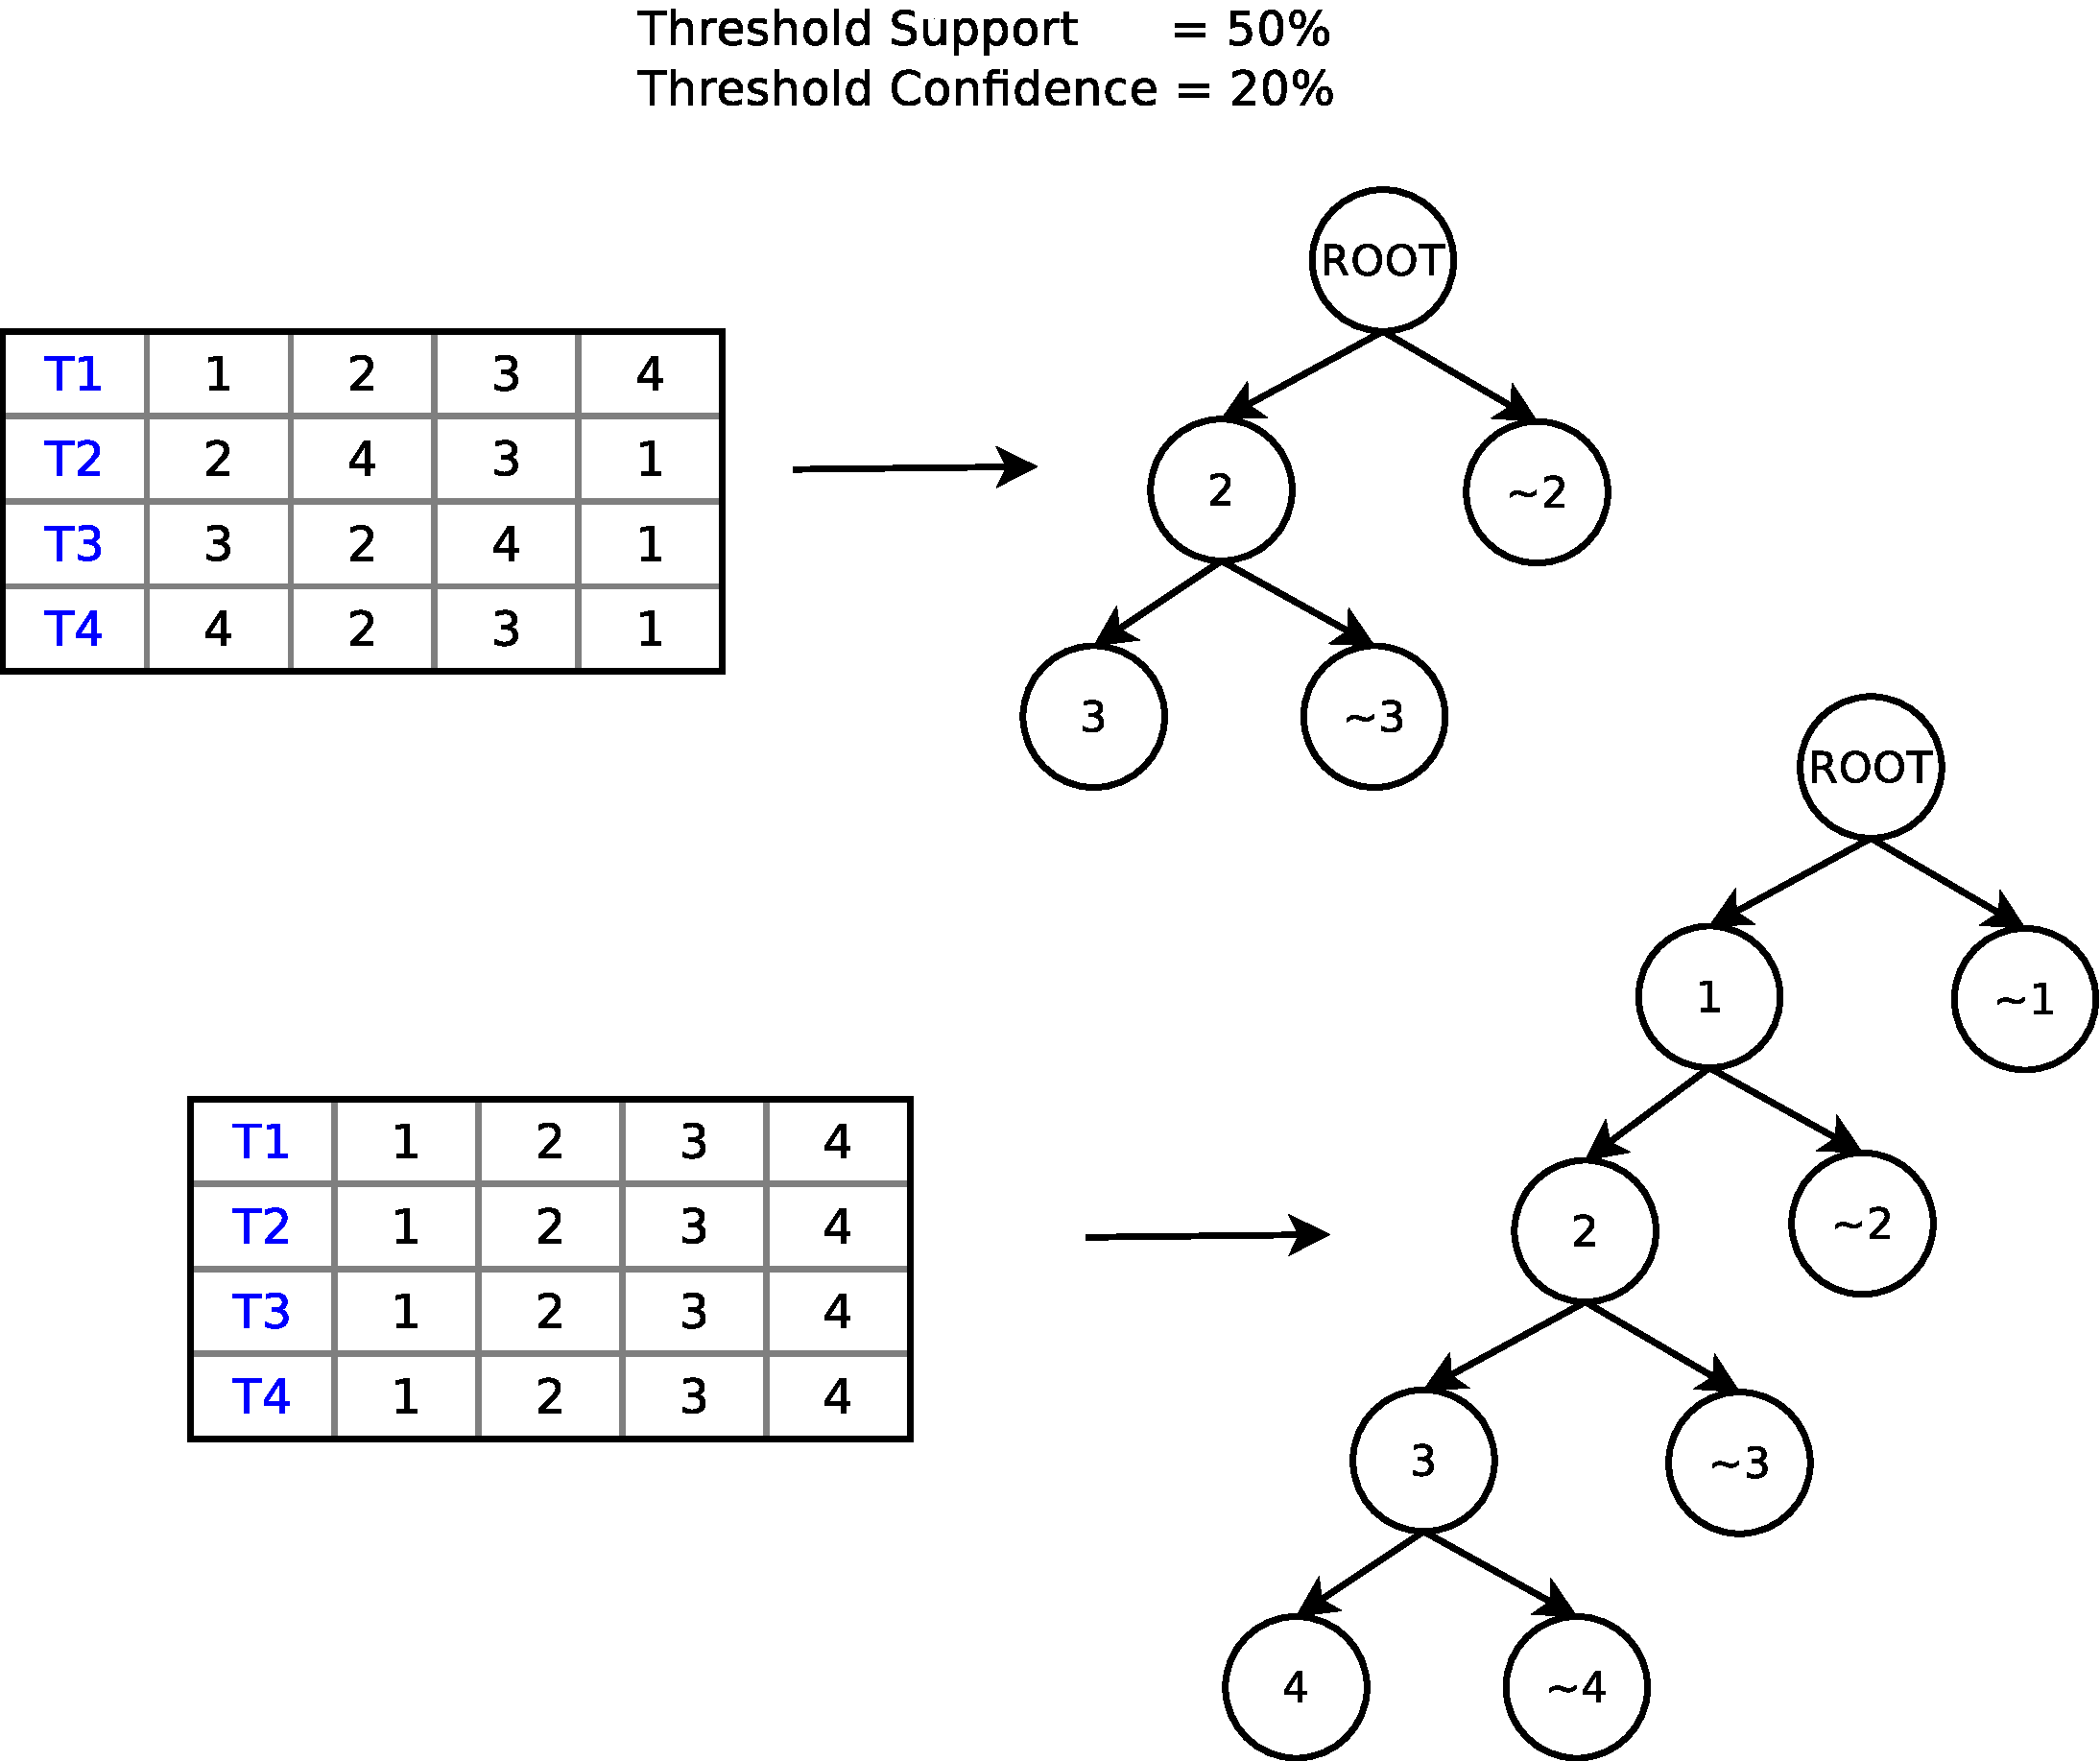
\includegraphics[scale=0.30]{pdf/firstimprove}
\end{center}
\caption{Differnt \emph{MASP} tree for the same dataset}
\label{Fig 12}
\end{figure}

This approach may produce different outcomes if we change the order of items in transactions. Figure \ref{Fig 12} shows this issue. We propose an approach which is order independent. An association rule of the form A $\Rightarrow$ B must satisfy the threshold support and threshold confidence i.e. probability of occurrence of A and B together must surpass threshold support, and the likelihood of occurrence of B in transactions containing A must be greater than or equal to threshold confidence. It means, to calculate support and confidence, it is required to traverse complete transaction database. What if an item appears for the first time in the $ ith $ transaction? It is biased to take the entire dataset for calculating support and confidence for the rules containing that particular item. So to generate all rules containing a particular item x, it is reasonable to ignore all transactions(for calculating support and confidence) that come before the transaction in which that particular item appears for the first time. Taking into account the origin of the item is the second proposed improvement. Embedding these two changes to the Omer M. Soyal \cite{oldmasp} approach is the basis of our research.

\section{Related works}
In 1994 R. Agrawal, et al. published non-trivial algorithm(Apriori) \cite{fastapriori} for finding association rules in large databases of the sales transaction. Apriori algorithm produces association rules in two steps. First generates all frequent itemsets(prune non-frequent candidate itemsets) and then make rules from those itemsets. This algorithm first finds frequent itemsets of length one then frequent itemsets of length 2 using frequent itemsets of length 1 and so on until generation of all frequent itemsets. This algorithm gave the better result than the previously known fundamental algorithms AIS \cite{ais}, SETM \citep{setm}. In 1996 Fukuda, et al. \cite{2darules} proposed an approach to find two-dimensional association rules. A state in this scenario is of the form ((X, Y) $\in$ P) $\Rightarrow$ (Z = z) where X and Y are numeric attributes, P is a subspace of 2-D plane, and Z is boolean attribute i.e. z can be either true or false. E.g. (Age $\in$ [30, 50] $\wedge$ Balance $\in$ [10$^{5}$, 10$^{6}$]) $\Rightarrow$ (CardLoan = yes). It means if a bank user age and balance lies in the given subspace it is very likely that they will use card loan. This approach works for specific types of structured data. R. Feldman, et al.(1997) \cite{massociation} introduced the notion of maximal association rules. These are the rules extracted from frequent maximal itemsets. Frequent maximal itemsets are those itemsets which appear just once among all transactions. It is useful in finding association rules containing negated attributes. As an example a rule \{milk, $\neg$bread\} $\Rightarrow$ \{$\neg$butter\} contains negated attributes. It means if a user purchases milk but not bread then the probability that the user will not buy butter is very high. This approach helps to capture inference rules which might be lost using regular associations. Till now items in transaction databases were treated uniformly. In 1998 C.H. Cai, et al. \cite{weightedassociation} gave an approach to find association rules which take into account weight(importance) of items in transaction databases. FP-Growth algorithm(2000) \cite{fpgrowth} also take two steps. The second phase is same as apriori. FP-Growth does not generate candidate frequent itemsets. First, it creates a tree(FP-Tree) and then finds frequent itemsets. This algorithm is about an order of magnitude faster than the Apriori algorithm. Lin, Weiyang, et al. \cite{Lin2002} proposed an approach that uses association rule mining for collaborative recommender systems. This approach does not require threshold support value. Instead, based on the number of rules(given) to be generated, threshold support is decided by the system. Thus it reduced the running time and produced enough rules for good recommendation performance. In 2004 F. Conen, et al. \cite{ptree} proposed two structures(T-Trees and P-Trees) which offer improvement concerning storage and execution time. In 2005 K. G. Srinivasa, et al. \cite{genetic} took advantage of genetic algorithms principles to generate large itemsets within dynamic transaction database. Their algorithm was better than the pre-existing FUP and E-Apriori concerning execution time and scalability. If transaction database is static, then life will be easy. In other scenario transaction database keeps on changing at high speed leading to change in data distribution. Hence it will be difficult to apply previously mentioned Association Rule Mining techniques. Jiang, et al.(2006) \cite{dynamicarm} came up with an approach to overcome this difficulty. In the same year G. Chen, et al. \cite{classify} used association rule mining for solving classification problems. It gave satisfactory results when compared to existing classification algorithms like C4.5, CBA, SVM, NN. Modification in traditional algorithm(apriori) was done \cite{bookrecommend} for building book recommendation system based on the data obtained from historical data of university library. Association rules having low support and high confidence are exception rules. In 2008 D. Taniar, et al. \cite{exceptionrules} proposed a new approach to finding exception rules. First, generate candidate exception rules and based on exceptionality measure obtain final ruleset. The quality of association rules depends on the threshold value of support and confidence. R.J. Kuo, et al.(2011) \cite{swarmarm} proposed an approach to find best threshold values which can produce quality rules. It gave promising results when compared to the genetic algorithm. Cloud computing provides an efficient and cheap way to store and analyze data. In 2011 L. Li, et al. \cite{cloudarm} proposed an effective strategy to perform association rule mining(frequent itemset mining) in cloud computing environment. Apriori \cite{fastapriori} generates candidate frequent itemsets before generating the desired itemsets. The modified algorithm(2012) \cite{minmizcandidt} minimizes the candidate itemsets generation. With the passage of time Association Rule Mining find its role in many applications. J. Nahar, et al.(2013) \cite{armheart} proposed a way to detect factors that can contribute to heart diseases in males and females. To enhance the quality of association rule mining researchers suggested to include factors such as value utility, temporal, etc. G. Maragatham, et al.(2015) \cite{utarm} have proposed an efficient algorithm which combines both utility and temporal time periods for mining extraordinary association rules. Their results show that UTARM(Utility-Based Temporal Association Rule Mining) algorithm efficiently discovers the utility-oriented temporal association rules. In 2016 O. M. Soysal, et al. \cite{sparseds} proposed a data structure for sparse memory allocation for parallel and sequential data mining. They have used this data structure on apriori-TID, MASP-tree, and FP-growth algorithms to reduce memory allocation cost. They concluded that the speed-up in apriori-TID is more than FP-growth and the modified MASP algorithm becomes 3.42 times faster than the old implementation \cite{oldmasp}.

\section{Method}
Let \emph{I} be a universal set of items. A single transaction($\tau$) is defined as a non empty subset of universal itemset(\emph{I}). Mathematically, $ \tau = \lbrace $ \textit{item}: \textit{item} $ \epsilon $ \emph{I} $\rbrace$. A \textit{transaction database}($ \Gamma $) is a collection of such transactions. A rule of the form \emph{X} $ \Rightarrow $ \emph{Y} is said to be derived from the transaction database $ \Gamma $ iff \emph{support}(\emph{X} $ \Rightarrow $ \emph{Y}) $ \geq \tau _{s} $(threshold support) and \emph{confidence}(\emph{X} $ \Rightarrow $ \emph{Y}) $ \geq \tau _{c} $(threshold confidence) where \emph{X} and \emph{Y} are non empty subsets of \emph{I} and \emph{X} $ \cap $ \emph{Y} $ =\phi $. What does \emph{support}(\emph{X} $ \Rightarrow $ \emph{Y}) mean? \emph{support}(\emph{X} $ \Rightarrow $ \emph{Y})  is defined as probability of occurence of \emph{X} and \emph{Y} together in the transaction database($ \Gamma $). Mathematically, \emph{support}(\emph{X} $ \Rightarrow $ \emph{Y}) $ = $ $ \frac{Count(X \cup Y)}{Count(\phi)} $ where \emph{Count(Z)} $ = $ Number of transactions in $ \Gamma $ which are superset of \emph{Z}. \emph{confidence}(\emph{X} $ \Rightarrow $ \emph{Y}) is the probabilty of occurence of \emph{Y} in those transactions of $ \Gamma $ which contains \emph{X} or \emph{confidence}(\emph{X} $ \Rightarrow $ \emph{Y}) $ = $ \emph{Probability(Y $ \vert $ X)} $ = $ $ \frac{Count(X \cup Y)}{Count(X)} $. Value of threshold support($ 0 \leq \tau _{s} \leq 1 $) and threshold confidence($ 0 \leq \tau _{c} \leq 1 $) is fixed before performing association rule mining.

First, we will explain how to generate \emph{OIMASP} tree before taking into account the origin of item in $ \Gamma $. Some of the terminologies that will be helpful in undersanding the algorithm.

\begin{enumerate}[1.]
\item A \textbf{transaction $ \tau $} is defined as collection of unique items.
\item A \textbf{transaction dataset $ \Gamma $} is a collection of many transactions. Constraints imposed on  transaction dataset
\begin{enumerate}[a)]
\item Evey transactions in the transaction database must have same number of items.
\item No duplicate items are allowed in rows of $ \Gamma $.
\end{enumerate}

\begin{figure}
\begin{center}
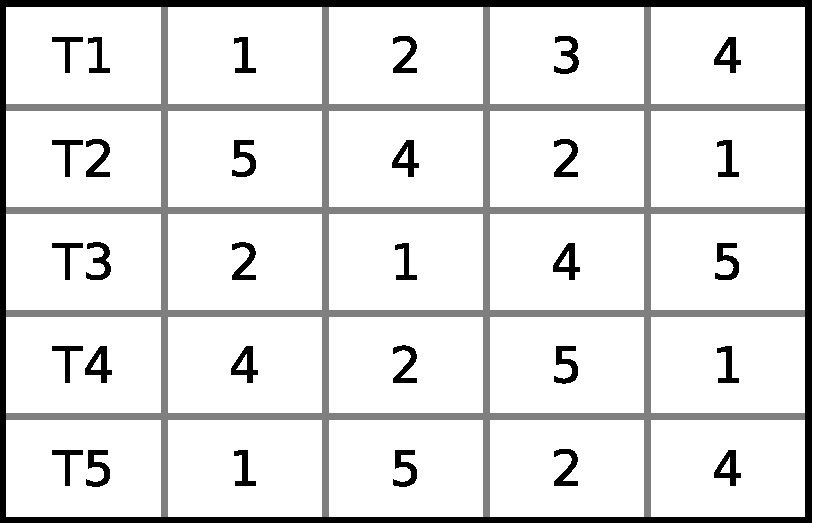
\includegraphics[scale=0.4]{pdf/validtrans}
\end{center}
\caption{Valid Transaction Dataset}
\label{Fig 1}
\end{figure}

\begin{figure}
\begin{center}
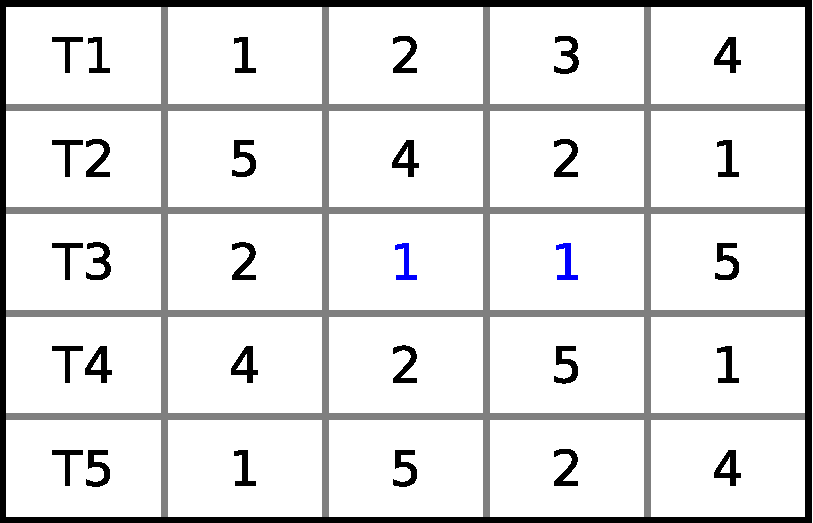
\includegraphics[scale=0.4]{pdf/invalidtrans}
\end{center}
\caption{Invalid Transaction Dataset}
\label{Fig 2}
\end{figure}

Transaction database \ref{Fig 1} is valid and \ref{Fig 2} is invalid(duplicate items(blue color) in \emph{T3}).

\item A sequence of items $ I = \{I_{1}, I_{2}, I_{3}, ..........., I_{n}\} $ will be an \emph{\textbf{OIMASP}} iff $ \forall $\emph{j} $ \in $ \{1, 2, ...., n\} the subset $ I' = \{I_{1}, I_{2}, ......., I_{j}\} $ must satisfy
\begin{enumerate}[i)]
\item $ support(I') \geq  \tau _{s} $
\item $P(I_{j} \vert I_{1}, I_{2}, ......., I_{j-1}) \geq \tau _{c}$
\item $P(I_{j} \vert I_{1}, I_{2}, ......., I_{j-1})$ is maximum.
\end{enumerate}

\item \textbf{Shuffle} is a function which takes transaction dataset, and an item as inputs and returns shuffled transaction dataset or \textbf{Shuffle}($ \Gamma $, \emph{I}) $ \rightarrow $ $ \Gamma _{shuffled} $. Shuffling is done in two steps
\begin{enumerate}[i)]

\begin{figure}
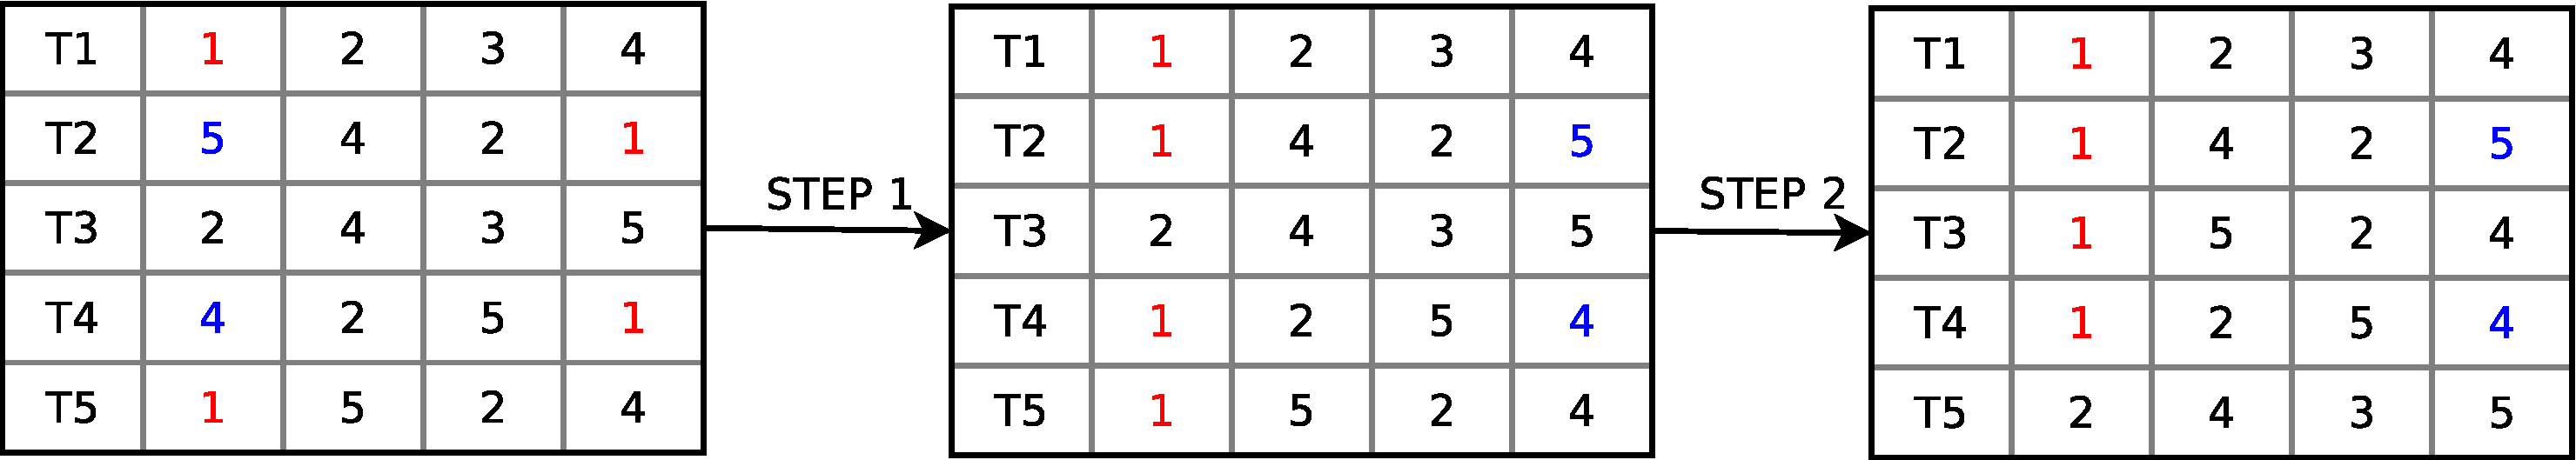
\includegraphics[scale=0.242]{pdf/shuffle}
\caption{Shuffling of dataset as per item \textbf{1}}
\label{Fig 3}
\end{figure}

\item $ \forall $ rows if the specified item(\emph{I}) is present in the row then perform swapping to bring that item to the first column \ref{Fig 3}.
\item Shuffle rows until there is no row left which contains item \emph{I} and appears below row which do not have item \emph{I} \ref{Fig 3}.
\end{enumerate}

\begin{figure}
\begin{center}
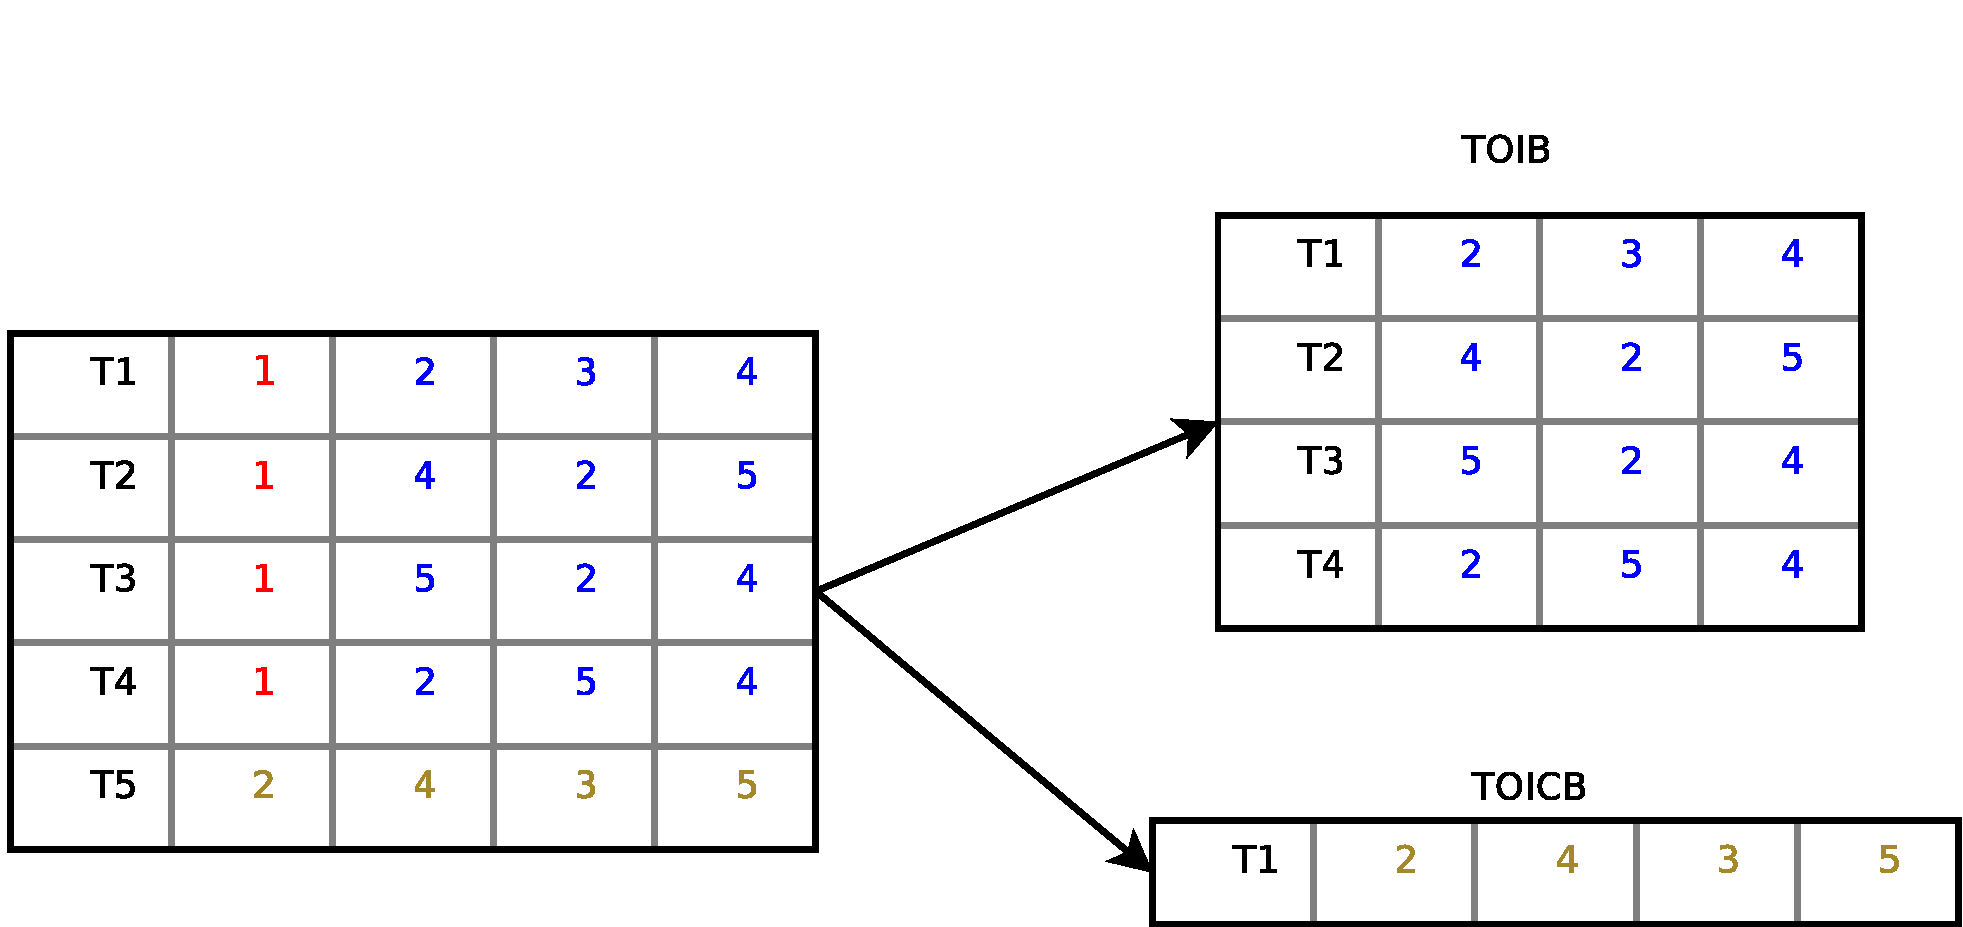
\includegraphics[scale=0.3]{pdf/tbtcb}
\end{center}
\caption{Splitting of $ \Gamma _{shuffled} $ into temporary order independent block and counter block}
\label{Fig 4}
\end{figure}

\item Temporary Order Independent Block(\textbf{TOIB}): After shuffling is done w.r.t the specified item, first obtain a subset of $ \Gamma _{shuffled} $ by taking transactions having specified item and then in the second step remove the first column. This newly received dataset is \textbf{TOIB} \ref{Fig 4}.

\item Temporary Order Independent Counter Block(\textbf{TOICB}): After shuffling is done w.r.t the specified item, the subset of $ \Gamma _{shuffled} $ obtained by taking transactions not having specified item is \textbf{TOICB} \ref{Fig 4}.

\item \emph{\textbf{OIB}}: It is defined for $ OIMASP = \{I_{1}, I_{2}, I_{3}, ..........., I_{k}\}  $.

\begin{algorithm}
    \SetKwInOut{Input}{Input}
    \SetKwInOut{Output}{Output}

    \underline{function generateOIB} $ (\Gamma, OIMASP, j) $\;
    \Input{A transaction dataset $ \Gamma $, $ OIMASP $ sequence and pointer $ j $ to current item}
    \Output{$ Order Independent Block $}
    \If{j points to the last element of $ OIMASP $}
      {
        return $ TOIB(\Gamma, OIMASP[j]) $\;
      }     
    \eIf{negation is present on jth item of $ OIMASP $}
      {
        $ temp \leftarrow TOICB(\Gamma, OIMASP[j]) $\;
		return $ generateOIB(temp, OIMASP, j+1) $
      }
      {
		$ temp \leftarrow TOIB(\Gamma, OIMASP[j]) $\;
		return $ generateOIB(temp, OIMASP, j+1) $
      }      
    \caption{Algorithm to generate Order Independent Block}
\end{algorithm}

\item Similarly \emph{\textbf{OICB}} is defined for $ OIMASP = \{I_{1}, I_{2}, I_{3}, ..........., I_{k}\}  $.

\begin{algorithm}
    \SetKwInOut{Input}{Input}
    \SetKwInOut{Output}{Output}

    \underline{function generateOICB} $ (\Gamma, OIMASP, j) $\;
    \Input{A transaction dataset $ \Gamma $, $ OIMASP $ sequence and pointer $ j $ to current item}
    \Output{$ Order Independent Block $}
    \If{j points to the last element of $ OIMASP $}
      {
        return $ TOICB(\Gamma, OIMASP[j]) $\;
      }     
    \eIf{negation is present on jth item of $ OIMASP $}
      {
        $ temp \leftarrow TOICB(\Gamma, OIMASP[j]) $\;
		return $ generateOICB(temp, OIMASP, j+1) $
      }
      {
		$ temp \leftarrow TOIB(\Gamma, OIMASP[j]) $\;
		return $ generateOICB(temp, OIMASP, j+1) $
      }      
    \caption{Algorithm to generate Order Independent Counter Block}
\end{algorithm}
\end{enumerate}

\subsection{How to generate OIMASP tree?}
In this section we have proposed an algorithm(OIMASP)[modified version of MASP \cite{oldmasp}] which is independent of the ordering of items in transactions of transaction database.

\begin{figure}
\begin{center}
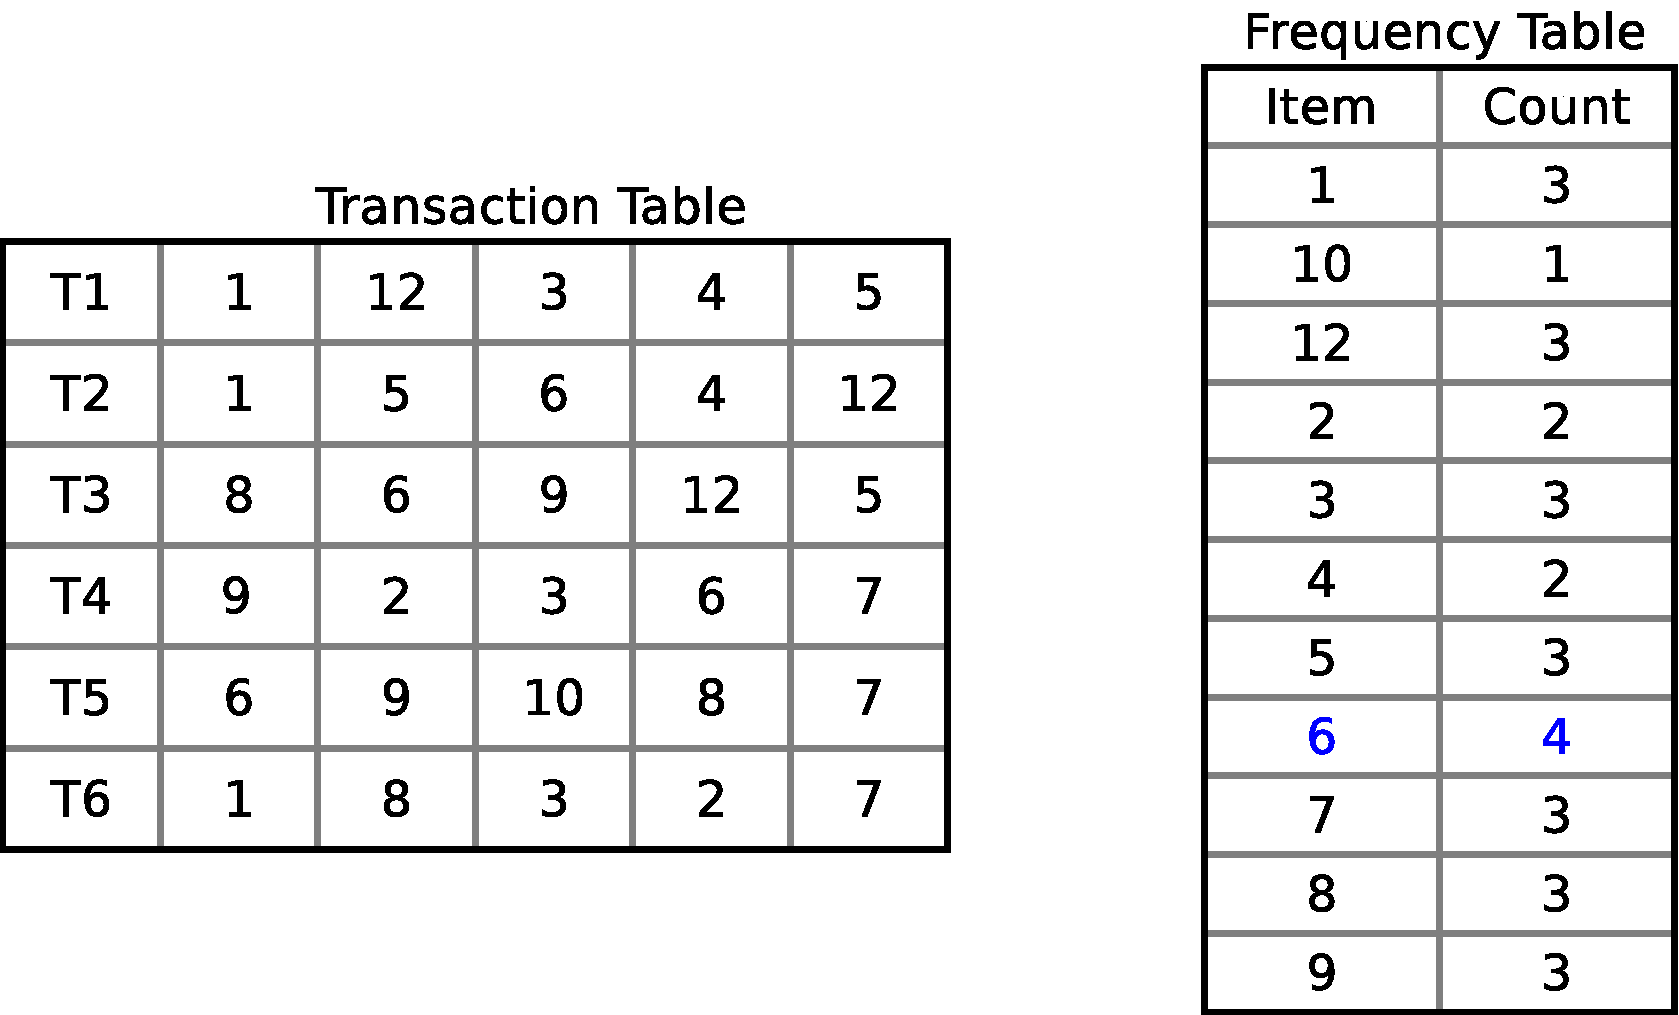
\includegraphics[scale=0.4]{pdf/itemfreq}
\end{center}
\caption{Transaction table on the left and items and their frequencies on the right}
\label{Fig 5}
\end{figure}

Initially we have the transaction table(\ref{Fig 5}), threshold support($ \tau _{s} $) $ = 0.2 $ and threshold confidence($ \tau _{c} $) $ = 0.3 $. Steps to generate OIMASP tree
\begin{enumerate}[Step 1.]
\item Initialize a tree having root node named as \emph{ROOT}. Transaction database associated with 
the root node is shown on the left in \ref{Fig 5}. Frequency table for the root node is shown on the right in \ref{Fig 5}.  Initially current node is the root node itself. Notation, $ \vert \Gamma \vert $ = number of rows in the transaction table associated with the root node and $ \vert \Gamma_{current} \vert $ = number of rows in the transaction table associated with the current node.
\item Draw the frequency table for the data associated with the current node.
\item Find the item having maximum frequency. Suppose item $ I $ is found to have the maximum frequency of $ f_{max} $.
\item If (support = $ \dfrac{f_{max}}{\vert \Gamma \vert} $) $ < \tau _{s} $ then return.
\item If (confidence = $ \dfrac{f_{max}}{\vert \Gamma_{current} \vert} $) $ < \tau _{c} $ then return.
\item Add a node on the left side of the current node. Name the new node(on the left) as $ I $ and associate data obtained from $ TOIB(\Gamma_{current}, I) $ with it.
\item Add a node on the right side of the current node. Name the new node(on the right) as $ ~I $ and associate data obtained from $ TOICB(\Gamma_{current}, I) $ with it.
\item Run Step 9 and Step 10 independently.
\item Mark the new node created in the Step 6 as the current node and then repeat from Step 2.
\item Mark the new node created in the Step 7 as the current node and then repeat from Step 2.
\item Return.
\end{enumerate}

\begin{figure}
\begin{center}
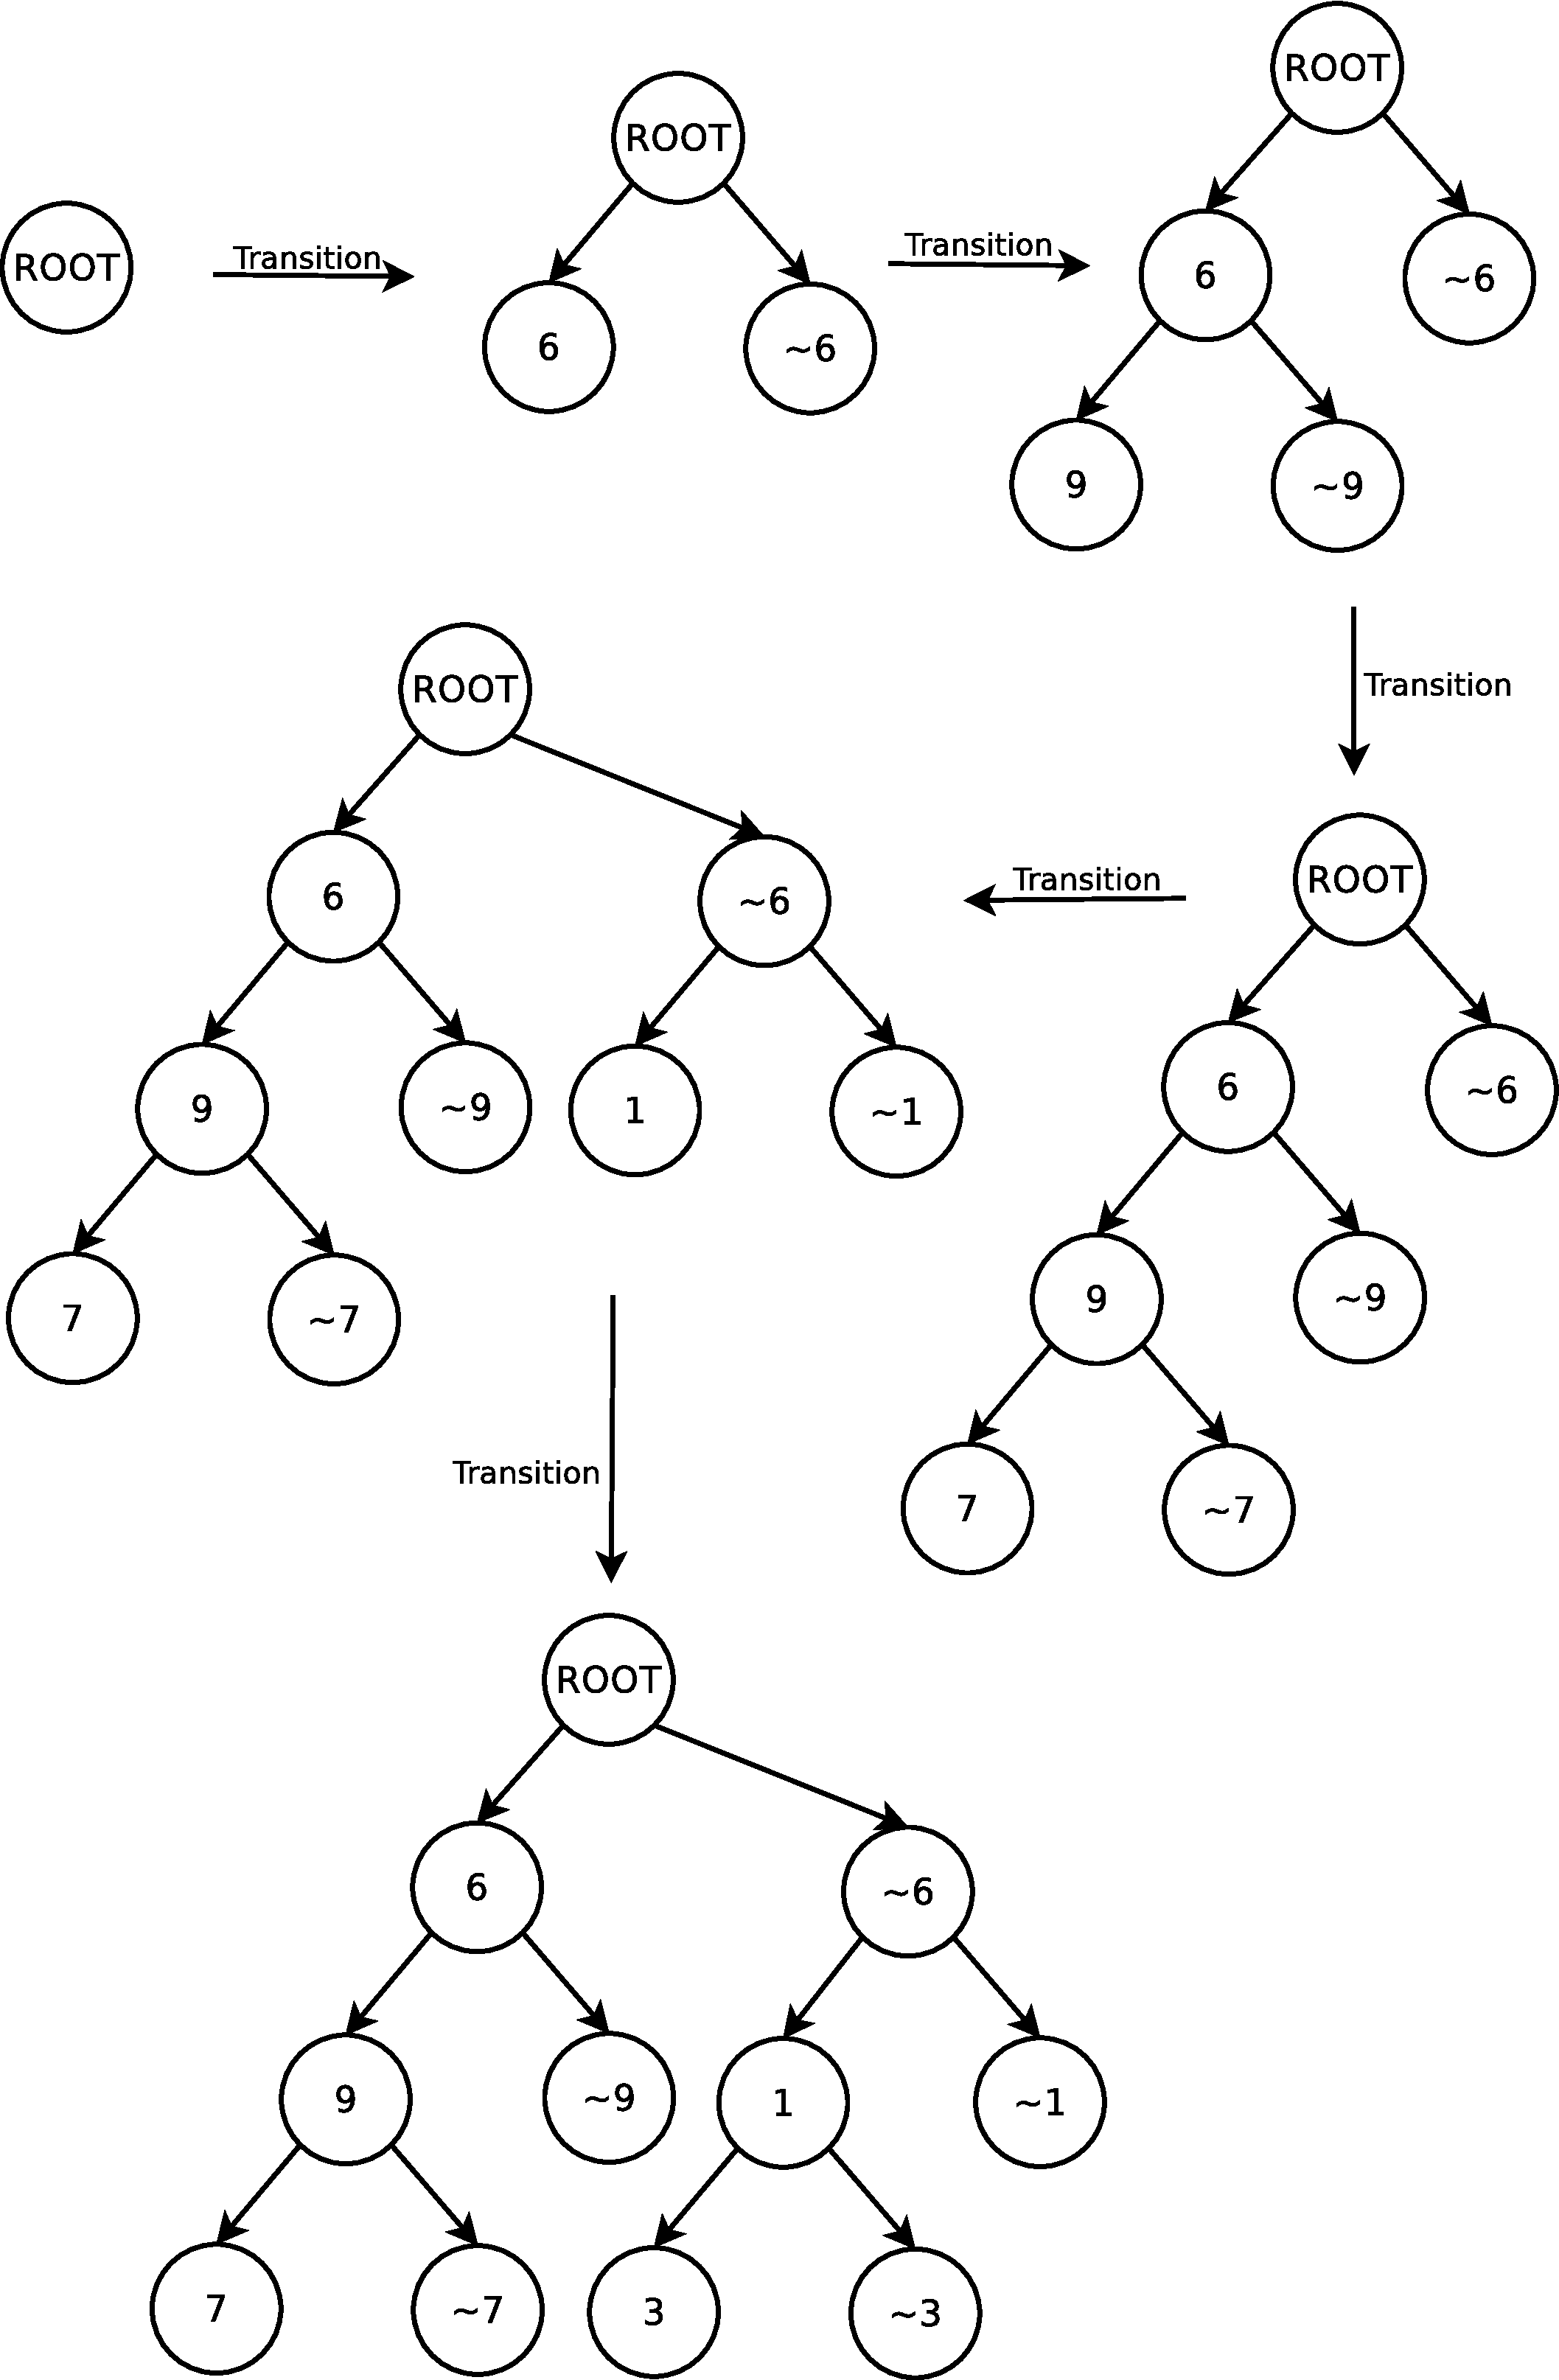
\includegraphics[scale=0.3]{pdf/transition}
\end{center}
\caption{Generation of OIMASP tree as the algorithm proceeds}
\label{Fig 6}
\end{figure}

If we apply the \emph{OIMASP} algorithm mentioned above for the transaction dataset shown in \ref{Fig 5}, threshold support($ \tau _{s} $) $ = 0.2 $ and threshold confidence($ \tau _{c} $) $ = 0.3 $, we will get the final \emph{OIMASP} tree in series of transitions as shown in \ref{Fig 6}.

\subsection{How to generate association rules out of OIMASP tree?}
\newdefinition{rmk}{Definition}
\begin{rmk}
	Given $ OIMASP = \{I_{1}, I_{2}, I_{3}, ..........., I_{k}\} $. Then $ \forall j $ $ \in $ $ \lbrace 2, 3, 4, 		..., k \rbrace $ $ (I_{1}, I_{2}, ..., I_{j-1})$ $ \Rightarrow (I_{j}) $ will be an association rule.		
\end{rmk}

A path from the root to the leaf of the \emph{OIMASP} tree will be an \emph{OIMASP}. Therefore, there can be multiple \emph{OIMASP}. An OIMASP and its corresponding association rules is shown in \ref{Fig 7}.

\begin{figure}
\begin{center}
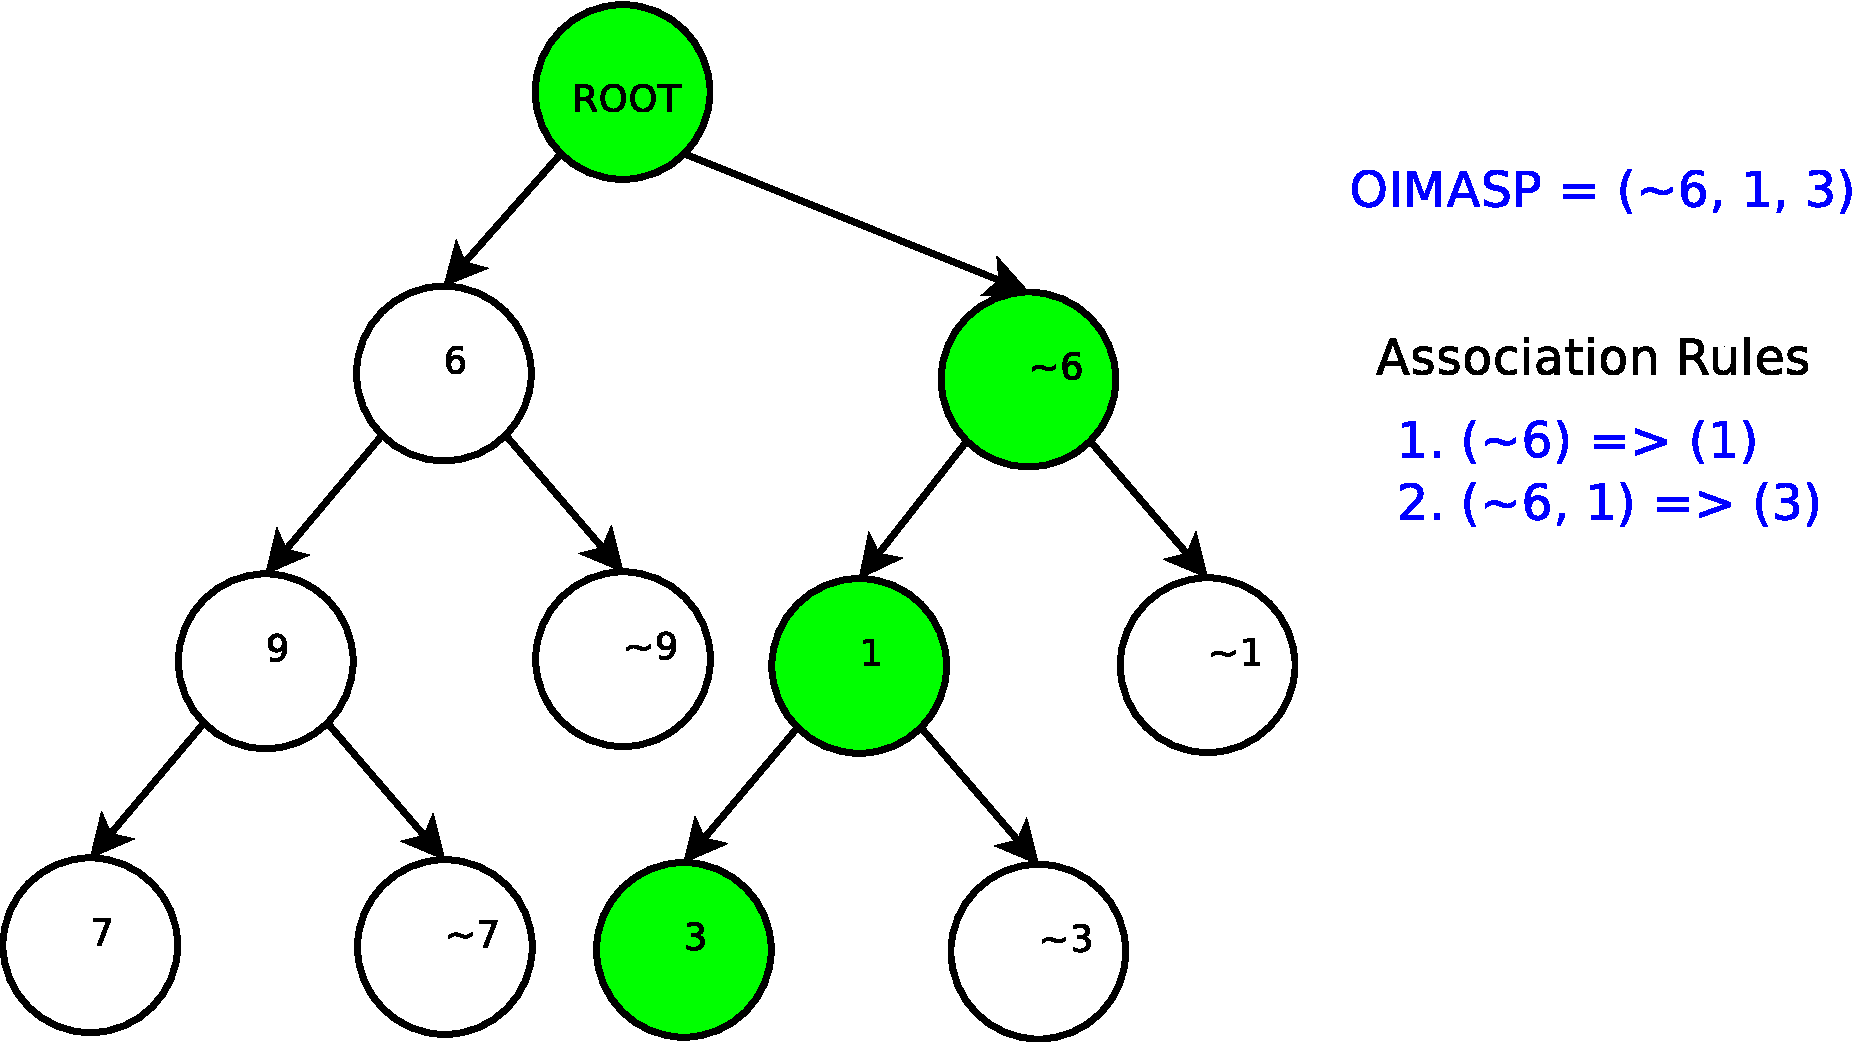
\includegraphics[scale=0.35]{pdf/oimasp}
\end{center}
\caption{An OIMASP(in green) and corresponding association rules}
\label{Fig 7}
\end{figure}

\subsection{Modified version of OIMASP(MOIMASP) which takes into account origins of items in the transaction database}
In this section, we will discuss the second modification to the \emph{MASP} algorithm proposed in \cite{oldmasp}. What if we want to generate those association rules which contains item $ I $? Our idea is to find the row starting from the top row of the transaction dataset in which item $ I $ appears for the first time(say $ ith $ row). Then for generating the $ OIMASP $ tree we will consider $ ith $ transaction and transactions afterward. Then generate all association rules and add only those rules to the solution set which contains item $ I $. It can be done for every unique element of $ \Gamma $ and finally take the union of solution sets obtained for each unique items to get the global solution set of association rules.

We will apply this algorithm for transaction dataset in (\ref{Fig 5}), threshold support($ \tau _{s} $) $ = 0.2 $, threshold confidence($ \tau _{c} $) $ = 0.3 $ and item $ = 10 $.

\begin{figure}
\begin{center}
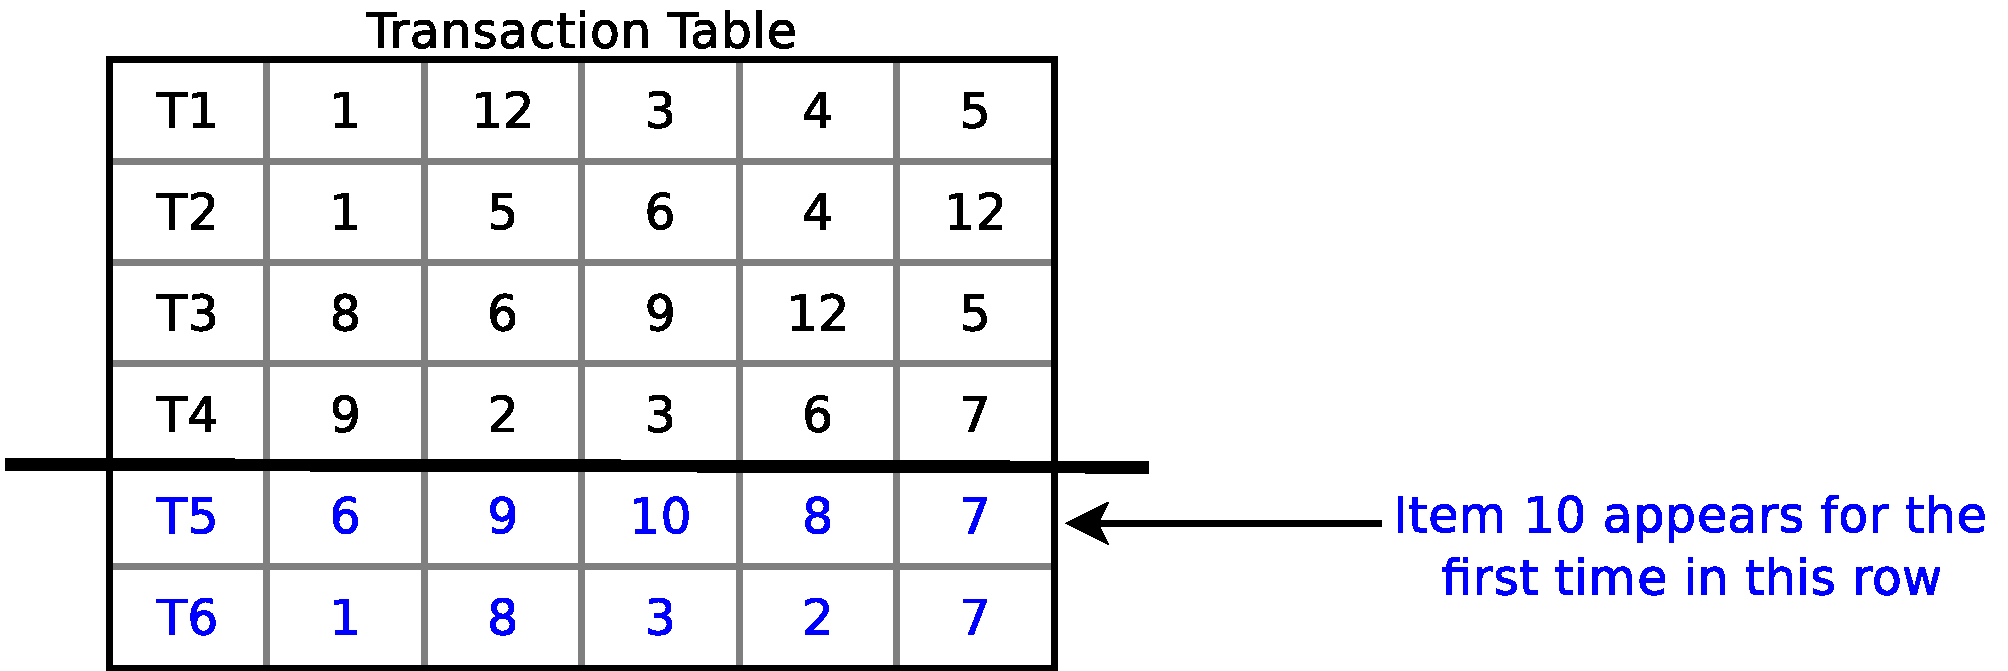
\includegraphics[scale=0.35]{pdf/partition}
\end{center}
\caption{Partition of dataset based on the origin of item $ 10 $}
\label{Fig 8}
\end{figure}

\begin{figure}
\begin{center}
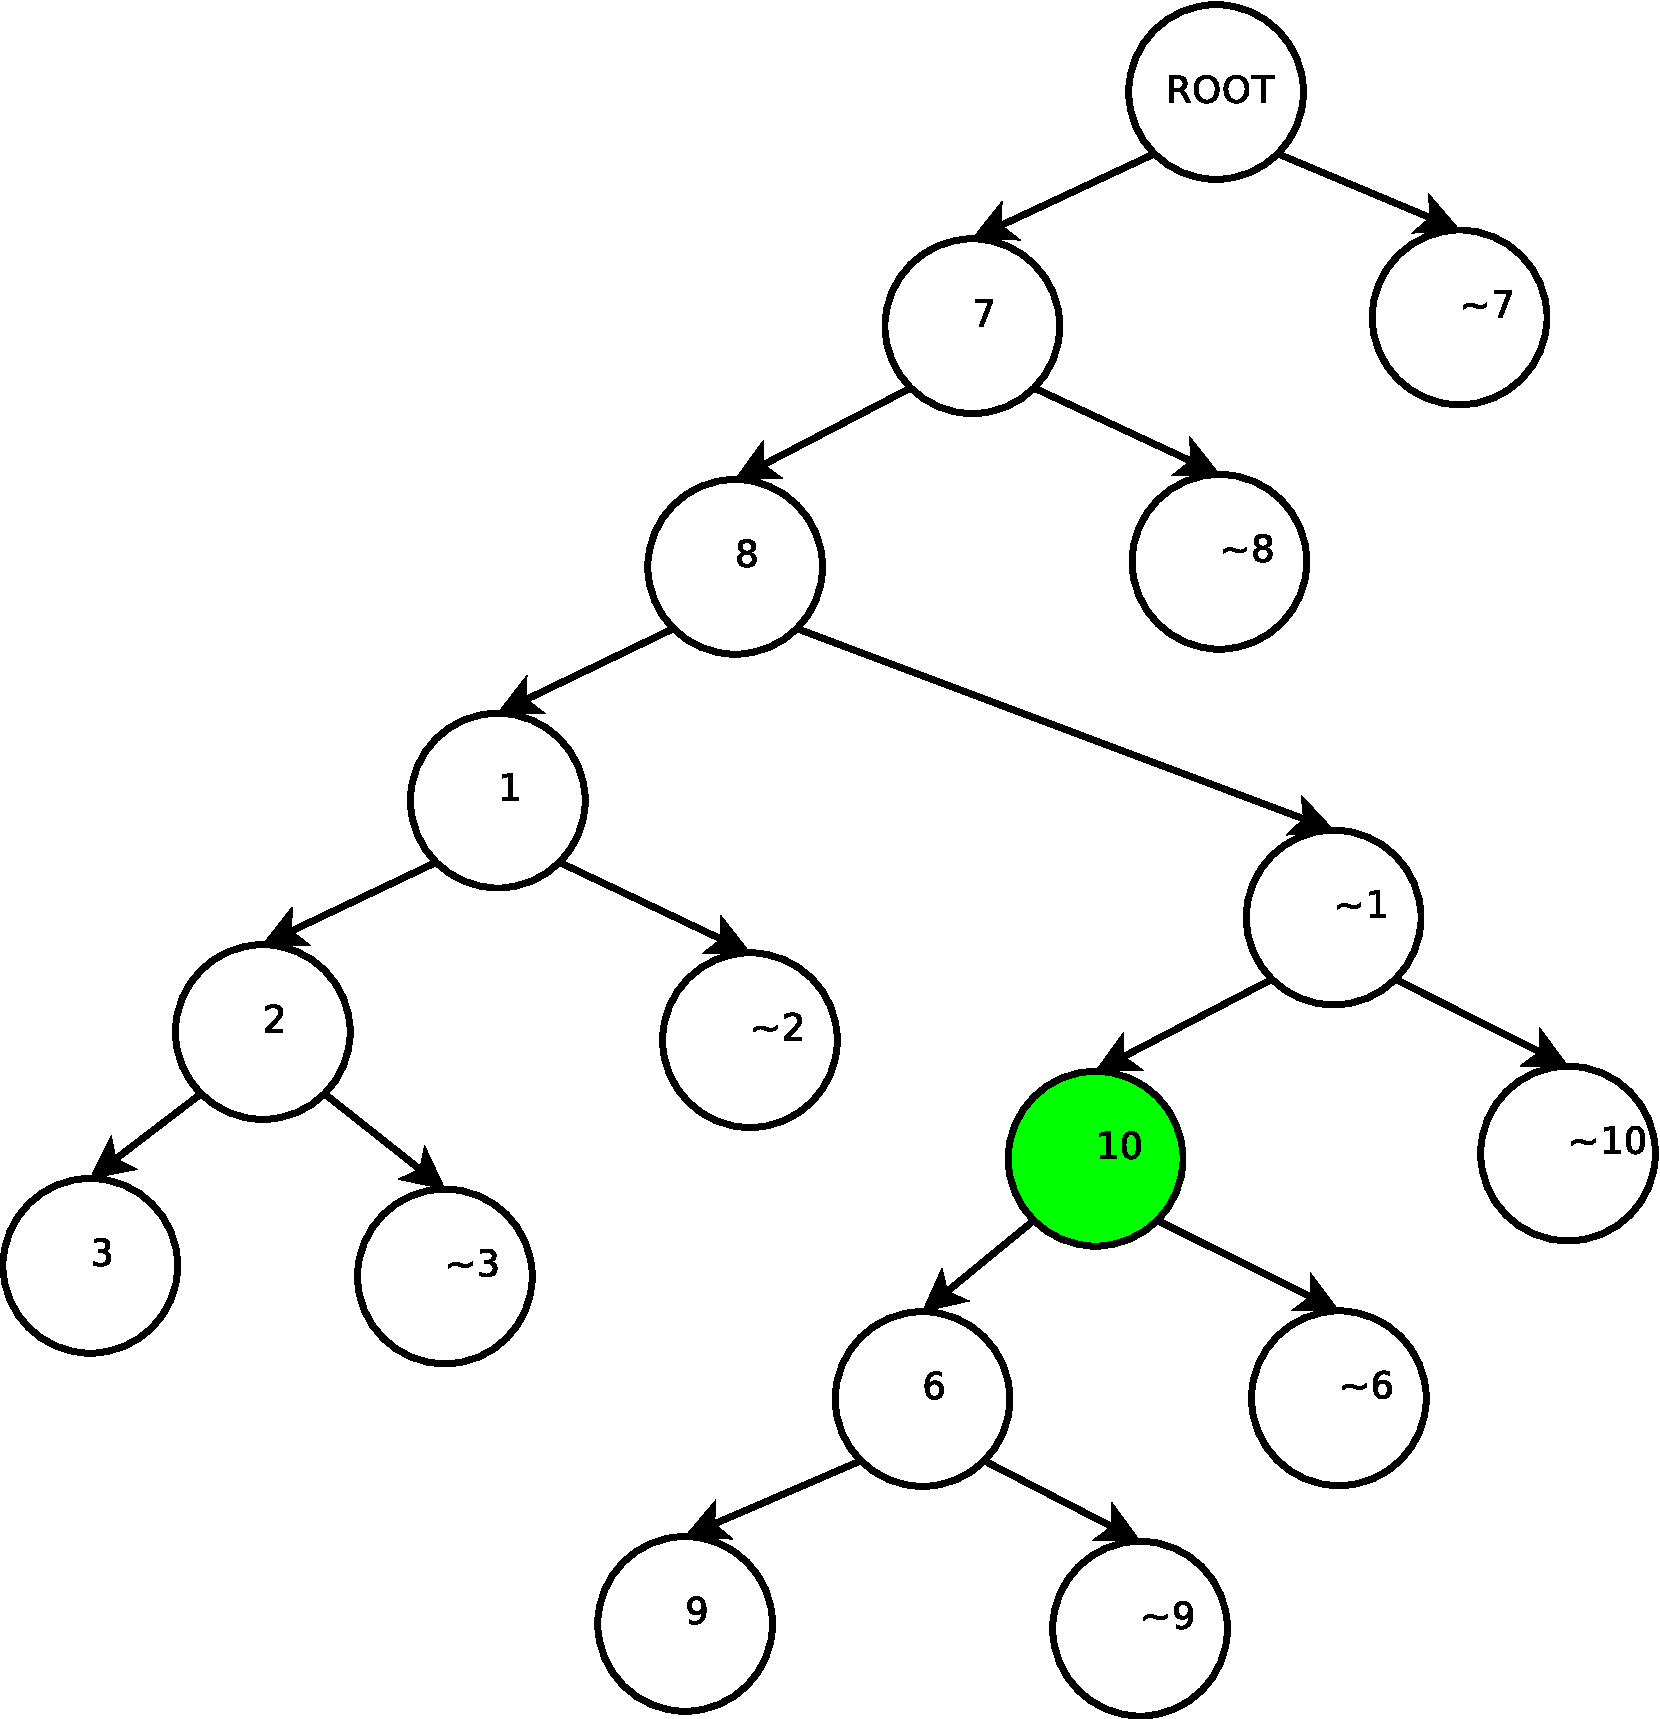
\includegraphics[scale=0.35]{pdf/moimasp}
\end{center}
\caption{An OIMASP tree}
\label{Fig 9}
\end{figure}

\begin{enumerate}[Step 1.]
\item A subdataset(consists of $ 5th $ and $ 6th $ row as shown in \ref{Fig 8}) is obtained based on the origin of item $ 10 $.
\item Apply \emph{OIMASP} tree generation algorithm on the new dataset to obtain \ref{Fig 9}.
\item Find association rules which conains item $ 10 $(see \ref{Fig 10}). Add rules obtained to the global solution set.
\item Repeat these steps for other items too.
\end{enumerate}

\begin{figure}
\begin{center}
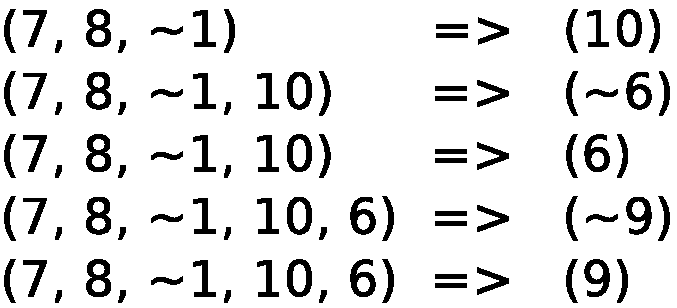
\includegraphics[scale=0.35]{pdf/arules10}
\end{center}
\caption{Association rules containing item $ 10 $}
\label{Fig 10}
\end{figure}

\textbf{Discussion:} If we generate $ OIMASP $ tree for all the items in the transaction database, then $ OIMASP $ tree generation algorithm will be called multiple numbers of times($ = $number of unique items in the dataset). It is possible that multiple items may have the same origin hence no need for redundancy(same $ OIMASP $ tree generation multiple times). Avoiding the redundancy can help us to less $ OIMASP $ tree production. In the worst case $ N $(total number of transactions) OIMASP tree will be generated.

\begin{algorithm}
    \SetKwInOut{Input}{Input}
    \SetKwInOut{Output}{Output}

    \underline{function MOIMASP} $ (\Gamma, \tau _{s}, \tau _{c}) $\;
    \Input{A transaction dataset $ \Gamma [N][M] $, threshold support $ \tau _{s} $ and 
	       threshold confidence $ \tau _{c} $}
    \Output{$ association\ rules $}
       
    $ items[1:j] $ $ \leftarrow $ unique items list \\
    $ origins[1:j] $ $ \leftarrow $ origin of corresponding items in $ items $ \\       
    $ globalRules \leftarrow \lbrace \rbrace $
       
	\For{i in 1 : j}
	  {
		$ currentItem $ $ \leftarrow $ $ items[i] $ \\
		$ itemOrigin $ $ \leftarrow $ $ origins[i] $ \\
			  	
	  	\If{$ OIMASP $ tree is not yet generated for origin $ itemOrigin $}
      	  {
            generate $ OIMASP $ tree for dataset $ = $ $ \Gamma[itemOrigin:N] $ and given $ \tau _{s} $, $ 				\tau _{c} $
          }	
          
		generate all association rules from $ OIMASP $ tree having origin $ = itemOrigin $, which contains 			item $ currentItem $ and add these to $ globalRules $
	  }
	          		
	return $ globalRules $;      
    \caption{MOIMASP Algorithm}
\end{algorithm}

\subsection{Complexity of MOIMASP algorithm}
The complexity of the \emph{MASP} algorithm \cite{oldmasp} is $ \Theta(NMlog(NM)) $. After the first improvement(OIMASP) complexity remains the same. In the final algorithm(\emph{MOIMASP}) \emph{OIMASP} can be called at max N times, so the complexity will be $ \displaystyle\sum_{i=1}^{N} \Theta(iMlog(iM)) = \Theta(N^{2}Mlog(NM)) $.

\section{Experiments and results}
The old approach and the new approach are compared using five datasets namely \href{https://github.com/cryptomanic/MOIMASP-datasets/blob/master/A.csv}{A}, \href{https://github.com/cryptomanic/MOIMASP-datasets/blob/master/B.csv}{B}, \href{https://github.com/cryptomanic/MOIMASP-datasets/blob/master/C.csv}{C}, \href{https://github.com/cryptomanic/MOIMASP-datasets/blob/master/D.csv}{D}, and \href{https://github.com/cryptomanic/MOIMASP-datasets/blob/master/E.csv}{E}. Metrics used for comparison are maximum rule size and the total number of rules generated. As you can see in \ref{Fig 11} that the new approach outperforms the old approach concerning number of rules generated and longest rule size. The amount of information obtained from the dataset has suppressed the increase in time complexity.

\begin{figure}
\begin{center}
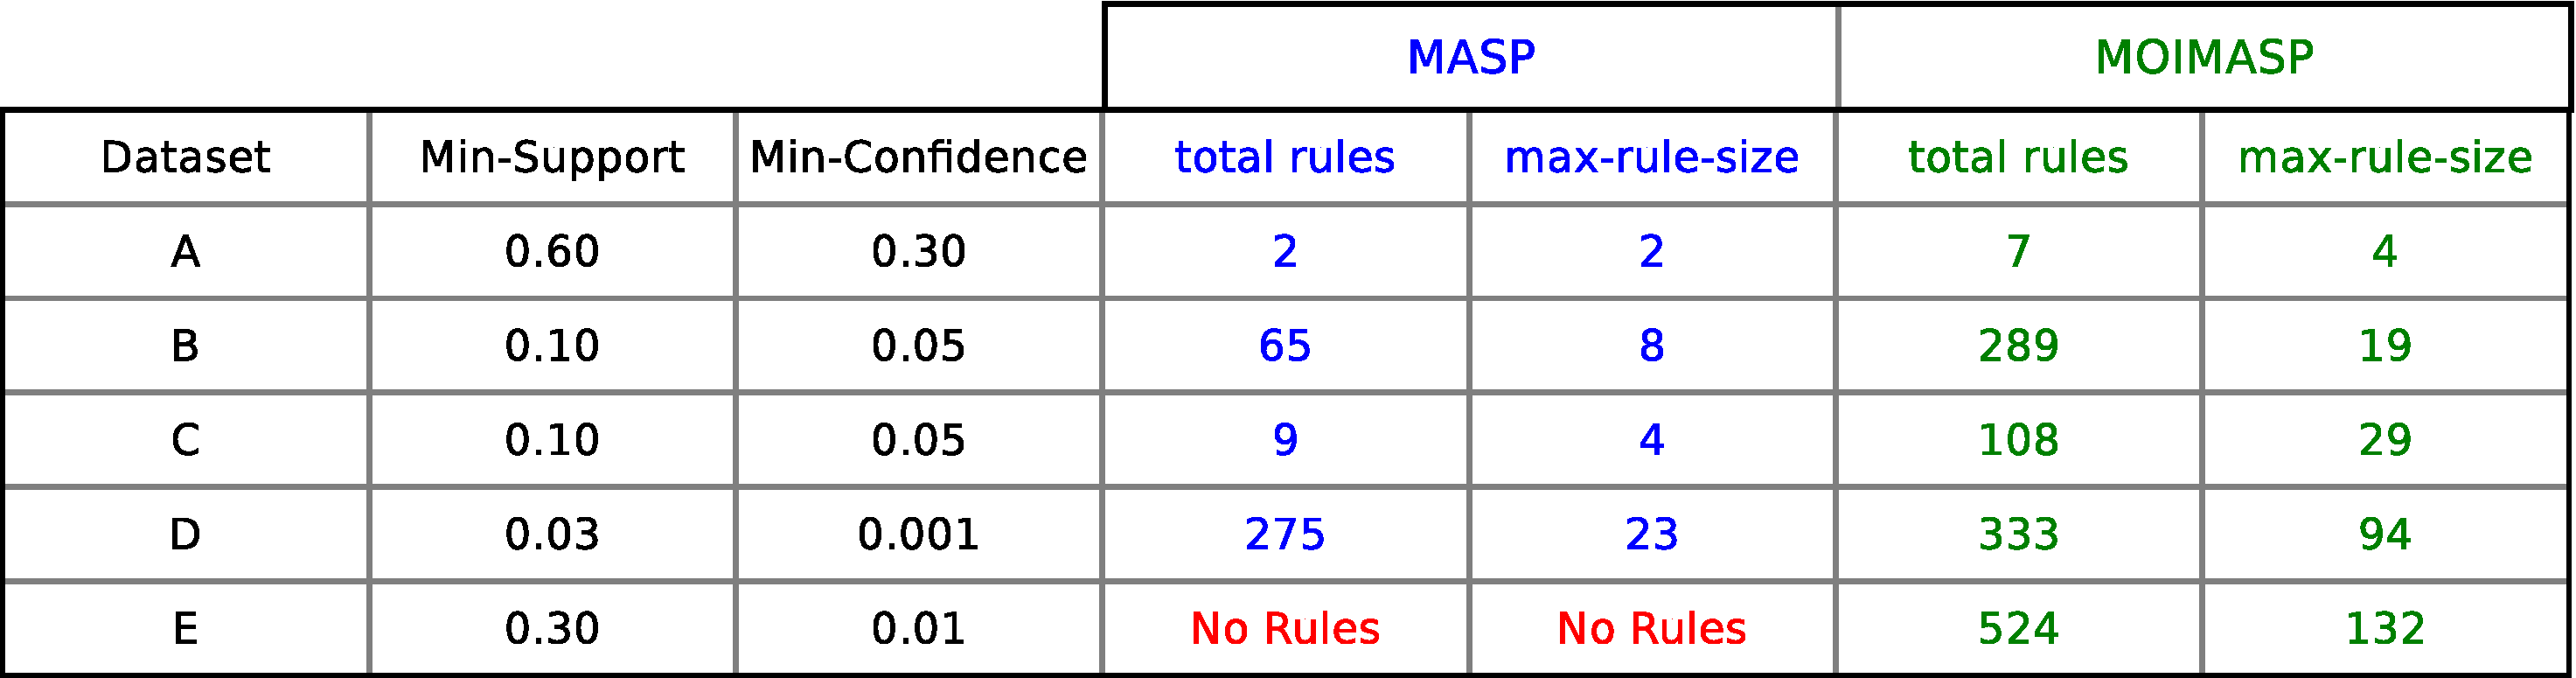
\includegraphics[scale=0.30]{pdf/comparison}
\end{center}
\caption{Comparison of \emph{MASP} and \emph{MOIMASP}}
\label{Fig 11}
\end{figure}

\section*{References}

\bibliography{mybibfile}

\end{document}